\documentclass{article}
    \usepackage{amssymb}
    \usepackage[utf8]{inputenc}
    \usepackage[russian]{babel}
    \usepackage[left=2cm,right=2cm,
        top=2cm,bottom=2cm,bindingoffset=0cm]{geometry}
    \usepackage{hyperref}
    \hypersetup{
        colorlinks=true,
        linkcolor=blue,
        filecolor=magenta,      
        urlcolor=cyan,
    }
  \usepackage{graphicx}
  \graphicspath{{pictures/}}
  \DeclareGraphicsExtensions{.pdf,.png,.jpg}
\usepackage{subcaption}
%\captionsetup{compatibility=false}

\begin{document}
\begin{center}{\hugeОтчет по курсовой работе за неделю\\}\end{center}
Дата: 3.12.2020\\
Научные руководители: Герасимов С.В., Мещеряков А.В.\\
Студент: Немешаева Алиса\\
Курс: 4\\

\renewcommand{\labelitemi}{$\blacksquare$}
\renewcommand\labelitemii{$\square$}
\begin{enumerate}
    \item На этой неделе основная работа велась по дополнению материалов для 
        \href{https://www.overleaf.com/read/zcgvtyscsyhv}{статьи}.\\
    \item Была заново обучена модель по каталогу planck\_z для построения графиков с кривыми 
        обучения (при первом обучении эти данные не сохранились).\\
        \begin{figure}[h]
            \center{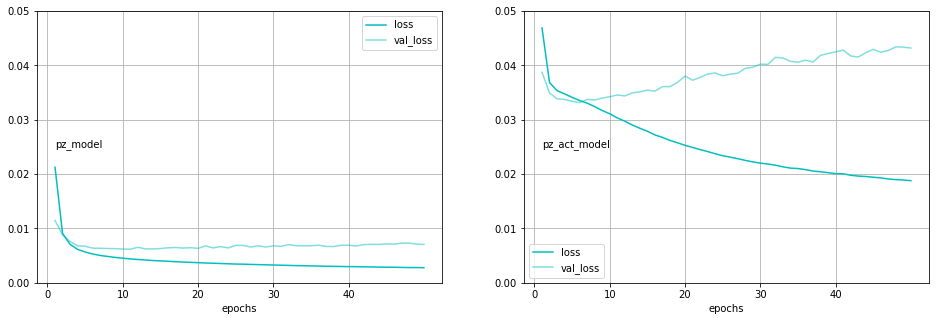
\includegraphics[width=0.7\linewidth]{loss}}
            \caption{Кривые обучения для моделей, обученных на каталогах planck\_z и planck\_z + act}
        \end{figure}
        \begin{figure}[h]
            \center{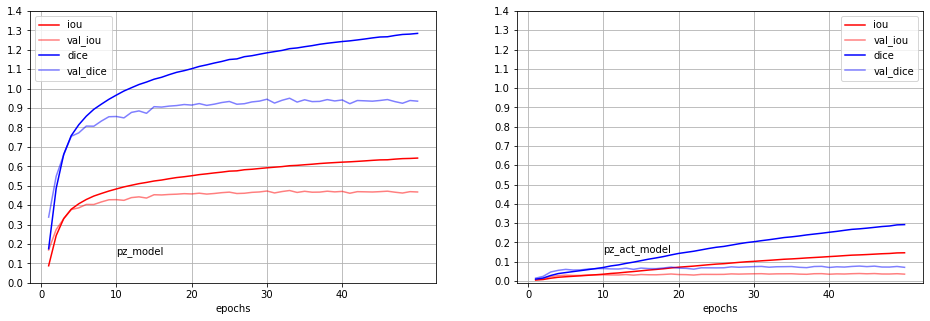
\includegraphics[width=0.7\linewidth]{iou_dice}}
            \caption{Кривые обучения для моделей, обученных на каталогах planck\_z и planck\_z + act}
        \end{figure}
    \item Для более подробного изучения параметра step (шаг окна сканирования при детекции) было 
        проведено сканирование валидационной области с новыми значениями этого параметра, которые 
        раньше не проверялись.\\
        \begin{figure}[h]
            \center{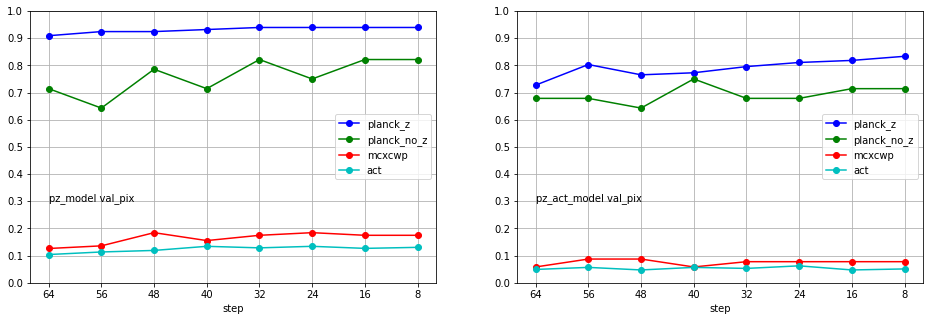
\includegraphics[width=0.7\linewidth]{recall_step}}
            \caption{Графики отклика по разным каталогам на валидационной области в зависимости от 
                параметра step}
        \end{figure}
        \begin{figure}[h]
            \center{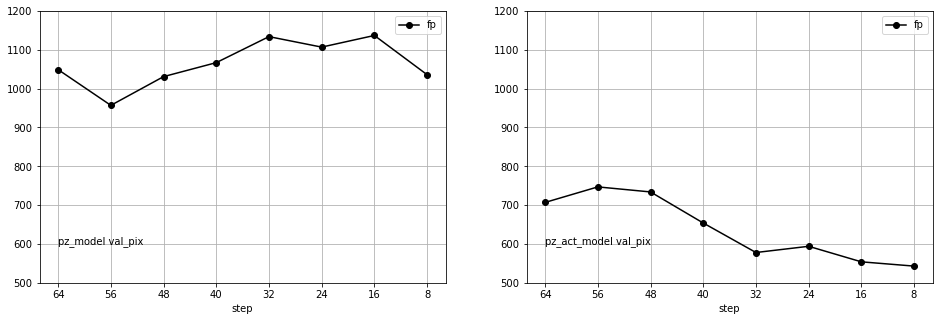
\includegraphics[width=0.7\linewidth]{fp_step}}
            \caption{Количество несопоставленных объектов на валидационной области в зависимости от 
                параметра step}
        \end{figure}
\end{enumerate}

Отчет согласован с научным руководителем.\\
Общее количество строк кода за эту неделю: 199\\
\href{https://github.com/rt2122/data-segmentation-2}{Репозиторий}\\ 
\end{document}
